\documentclass[11pt]{article}
\usepackage[margin=1in]{geometry}
\usepackage{booktabs}
\usepackage{graphicx}
\usepackage{amsmath}
\usepackage[numbers]{natbib}
\usepackage[hidelinks]{hyperref}
\graphicspath{{figs/}}
\newcommand{\ArmASrOne}{0.333}
\newcommand{\ArmACntOne}{32}
\newcommand{\ArmASrTwo}{0.250}
\newcommand{\ArmACntTwo}{24}
\newcommand{\ArmASrThree}{0.198}
\newcommand{\ArmACntThree}{19}
\newcommand{\ArmASrFour}{0.031}
\newcommand{\ArmACntFour}{3}
\newcommand{\ArmASrFive}{0.031}
\newcommand{\ArmACntFive}{3}
\newcommand{\ArmAs}{0.484}
\newcommand{\ArmAsLo}{0.193}
\newcommand{\ArmAsHi}{0.589}
\newcommand{\ArmAHalfLife}{0.95}
\newcommand{\ArmBSrOne}{0.729}
\newcommand{\ArmBCntOne}{70}
\newcommand{\ArmBSrTwo}{0.417}
\newcommand{\ArmBCntTwo}{40}
\newcommand{\ArmBSrThree}{0.125}
\newcommand{\ArmBCntThree}{12}
\newcommand{\ArmBSrFour}{0.083}
\newcommand{\ArmBCntFour}{8}
\newcommand{\ArmBSrFive}{0.083}
\newcommand{\ArmBCntFive}{8}
\newcommand{\ArmBs}{0.573}
\newcommand{\ArmBsLo}{0.208}
\newcommand{\ArmBsHi}{0.733}
\newcommand{\ArmBHalfLife}{1.24}
\newcommand{\ArmCSrOne}{1.000}
\newcommand{\ArmCCntOne}{96}
\newcommand{\ArmCSrTwo}{1.000}
\newcommand{\ArmCCntTwo}{96}
\newcommand{\ArmCSrThree}{1.000}
\newcommand{\ArmCCntThree}{96}
\newcommand{\ArmCSrFour}{1.000}
\newcommand{\ArmCCntFour}{96}
\newcommand{\ArmCSrFive}{1.000}
\newcommand{\ArmCCntFive}{96}
\newcommand{\ArmCs}{1.000}
\newcommand{\ArmCsLo}{1.000}
\newcommand{\ArmCsHi}{1.000}
\newcommand{\ArmCHalfLife}{$\infty$}
\newcommand{\TotalCost}{3.38}
\newcommand{\MeanLatency}{14.4}
\newcommand{\NCalls}{105}
\newcommand{\NMutated}{0}
\newcommand{\ArmAMeanWords}{99}
\newcommand{\ArmAOverBudget}{1}
\newcommand{\ArmBMeanWords}{214}
\newcommand{\ArmBOverBudget}{0}
\newcommand{\ArmCMeanWords}{119}
\newcommand{\ArmCOverBudget}{3}
\newcommand{\PilotRoneRetention}{0.938}
\newcommand{\NProbed}{18}
\newcommand{\NProbeRetained}{1}
\newcommand{\NProbeRetainedExact}{1}
\newcommand{\NProbeLost}{17}
\newcommand{\NProbeAbstained}{17}
\newcommand{\NProbeConfab}{0}
\newcommand{\ProbeCost}{0.14}
\newcommand{\GrandCost}{3.52}
\newcommand{\HTwoRfiveDiff}{+0.052}
\newcommand{\HTwoRfiveLo}{-0.062}
\newcommand{\HTwoRfiveHi}{+0.250}
\newcommand{\HTwoSDiff}{+0.089}
\newcommand{\HTwoSLo}{-0.320}
\newcommand{\HTwoSHi}{+0.460}
\newcommand{\HThreeRfiveDiff}{+0.969}
\newcommand{\HThreeRfiveLo}{+0.906}
\newcommand{\HThreeRfiveHi}{+1.000}
\newcommand{\HThreeSDiff}{+0.516}
\newcommand{\HThreeSLo}{+0.411}
\newcommand{\HThreeSHi}{+0.807}
\newcommand{\CBRfiveDiff}{+0.917}
\newcommand{\CBRfiveLo}{+0.750}
\newcommand{\CBRfiveHi}{+1.000}


\title{The Compaction Half-Life: Measuring Fact Survival\\Under Iterated Context Summarization}
\author{Yash Singh\\\small IIIT Una}
\date{July 19, 2026}

\begin{document}
\maketitle

\begin{abstract}
Long-running LLM agents periodically compress their working context into a
summary and continue from the summary alone. I measure how fast discrete facts
decay under this iterated compaction. In each chain, 16 atomic facts (8-character
codes with plain-language descriptors) are planted in a roughly 3{,}000-word task
log; the model compresses the log to a word budget, receives roughly 1{,}200 words
of fact-free distractor activity, and re-compresses, for 5 rounds. I run 3
pre-registered arms (6 chains each, 90 calls) on a small production model:
a 150-word budget, a 400-word budget, and a 150-word budget plus a one-line
instruction to preserve identifiers verbatim. Retention decays quickly under
plain instructions: round-5 survival is \ArmASrFive{} (150-word arm) and
\ArmBSrFive{} (400-word arm), with fitted per-round survival $s=\ArmAs$ and
$s=\ArmBs$, i.e.\ a compaction half-life of roughly \ArmAHalfLife{} and
\ArmBHalfLife{} rounds. The verbatim-preservation instruction dominates both:
all 96 planted codes survive all 5 rounds ($S(5)=\ArmCSrFive$), a pre-registered
difference of $\HThreeRfiveDiff$ round-5 survival over the plain 150-word arm
(95\% CI $[\HThreeRfiveLo,\HThreeRfiveHi]$). The 2.7$\times$ larger budget alone
produced no claimable round-5 difference. Loss is availability, not corruption:
\NMutated{} near-miss mutations of planted codes were observed in any summary,
and in probe tests lost facts led to abstention (\NProbeAbstained/\NProbeLost),
never confabulated codes. A one-line prompt change, not a bigger summary budget,
was the decisive lever for fact survival under compaction.
\end{abstract}

\section{Introduction}

Agentic LLM systems outlive their context windows. Coding agents, support
agents, and long-horizon research agents all eventually compress their working
history into a summary and continue from the summary alone, often many times in
a single session. Each compaction is lossy, and losses compound: a fact dropped
at round 2 is unavailable at every later round. Prior work has documented how
performance degrades as context grows \cite{hong2025contextrot} and how models
lose information across multi-turn interaction \cite{laban2025lost}, but the
decay rate of specific, verifiable facts under \emph{iterated} summarization
has received less direct measurement.

This paper asks three pre-registered questions. \textbf{H1 (shape):} does fact
survival decay geometrically (a constant per-round survival probability), or is
loss front-loaded in the first compaction? \textbf{H2 (budget):} does a larger
summary budget (400 words vs.\ 150) slow decay? \textbf{H3 (instruction):} does
a one-line instruction to preserve identifiers verbatim slow decay?

The design is deliberately minimal: facts are random 8-character codes attached
to operational descriptors (for example, a deploy ticket reference), planted in
realistic task-log filler, and scored by verbatim substring match in each
round's summary. This makes retention binary, machine-checkable, and immune to
scoring ambiguity. All rules, budgets, and decision criteria were fixed in a
config file before the main run.

Findings in brief: decay under plain compaction instructions is severe (fitted
half-life of roughly \ArmAHalfLife{}--\ArmBHalfLife{} rounds); the shape is
statistically consistent with geometric decay at this sample size; the larger
budget produced no claimable benefit at round 5, while the verbatim-preservation
instruction produced perfect retention through all 5 rounds. Failure mode
matters too: facts vanish cleanly rather than getting corrupted, and the model
abstains rather than confabulating when asked about lost facts.

\section{Related Work}

\citet{liu2024lost} showed that models use long contexts unevenly, with
positional (lost-in-the-middle) effects on retrieval. \citet{hong2025contextrot}
measured performance degradation as input length grows even on simple tasks.
\citet{laban2025lost} found large average drops in multi-turn settings, driven
substantially by unreliability rather than aptitude, which parallels the large
run-to-run variance observed here. On the constructive side, agent-memory
systems compress and manage context deliberately: Mem0 \cite{chhikara2025mem0}
builds production long-term memory via extraction and consolidation, Dynamic
Cheatsheet \cite{suzgun2025dynamic} maintains an adaptive test-time memory, and
agentic context engineering \cite{zhang2025agentic} evolves contexts to improve
them over time. This paper complements that line by quantifying the default
loss rate such systems must beat, and by isolating a cheap prompt-level lever
(verbatim preservation) that changes the decay constant dramatically.

\section{Method}

\paragraph{Chains.} A chain is 5 sequential summarize-and-continue rounds.
Round 1 presents an instruction plus a roughly 3{,}000-word synthetic task log
(the source). Each later round presents the instruction, the previous round's
summary, and a fresh roughly 1{,}200-word fact-free distractor segment
describing continued activity. The model outputs only the compressed context.

\paragraph{Facts.} Each chain plants 16 atomic facts of the form ``The
$\langle$descriptor$\rangle$ is $\langle$CODE$\rangle$'' at controlled positions
in the source. Codes are random 8-character strings from an alphabet that
excludes ambiguous characters (no 0/O or 1/I/L), so substring scoring is
unambiguous. Descriptors are operational (ticket references, dashboard UIDs,
tokens, and similar). All content is seeded and recorded.

\paragraph{Arms.} Three arms, 6 chains each, sharing content seeds across arms
so arm contrasts compare identical facts and filler. Arm A: ``Compress the
following working context into at most 150 words, preserving everything needed
to continue the task.'' Arm B: identical with a 400-word budget. Arm C: the Arm
A instruction plus one sentence: ``Preserve all identifiers, codes, numbers,
and proper nouns verbatim.''

\paragraph{Model and calls.} The model under test is a small production model
(Claude Haiku class) called through a headless CLI with JSON output; every raw
response is retained on disk. The main run is $3 \times 6 \times 5 = 90$ calls.
A 5-call pilot chain calibrated difficulty before the main run (pre-registered
gate: round-1 retention in $[0.15, 0.95]$; observed \PilotRoneRetention, so the
main run proceeded unchanged). Six validation probe calls and a 10-call
spot-repeat (the A-0 chain spec run twice more) complete the budget. In total
\NCalls{} chain calls and \NProbed{} probed facts are analyzed; total cost was
USD~\GrandCost{} with mean per-call API latency \MeanLatency{}s.

\paragraph{Scoring (pre-registered).} A fact survives round $r$ if its code
appears verbatim (case-insensitive substring, whitespace normalized) in the
round-$r$ summary. Corruption is scored separately: any 6--10 character
alphanumeric token in a summary at Levenshtein distance 1--2 from a planted
code that is absent verbatim counts as a mutated code. Geometric fits use least
squares of $\log S(r) = r \log s$ through the origin on arm-level chain-mean
survival; half-life is $\ln 2 / (-\ln s)$. The decay shape rule computes
conditional survival $c_r = S(r)/S(r-1)$ and $\delta = c_1 -
\operatorname{mean}(c_2..c_5)$; decay is called front-loaded only if the 95\%
bootstrap CI of $\delta$ (resampling chains, 10{,}000 reps) excludes 0 with
$\delta < 0$. Arm contrasts are claimed only if the 95\% bootstrap CI of the
difference excludes 0. All rules were fixed before the main run; every number
in this paper is emitted by the analysis pipeline from the raw response files.

\section{Results}

\subsection{Survival curves and half-life}

Table~\ref{tab:survival} and Figure~\ref{fig:retention} give the headline
result. Under the plain 150-word instruction (Arm A), only \ArmACntOne{} of 96
codes survive even one compaction ($S(1)=\ArmASrOne$), and \ArmACntFive{} of 96
survive round 5. The 400-word budget (Arm B) starts much higher
($S(1)=\ArmBSrOne$) but converges toward the same floor by round 3
($S(3)=\ArmBSrThree$ vs.\ \ArmASrThree). Fitted per-round survival is
$s=\ArmAs$ $[\ArmAsLo,\ArmAsHi]$ for Arm A and $s=\ArmBs$
$[\ArmBsLo,\ArmBsHi]$ for Arm B: a compaction half-life of roughly
\ArmAHalfLife{} and \ArmBHalfLife{} rounds respectively. Arm C is at the
measurement ceiling: all 96 codes survive all 5 rounds
($S(5)=\ArmCSrFive$, $s=\ArmCs$), so its half-life is unresolvable within this
horizon (reported as \ArmCHalfLife).

\begin{figure}[t]
\centering
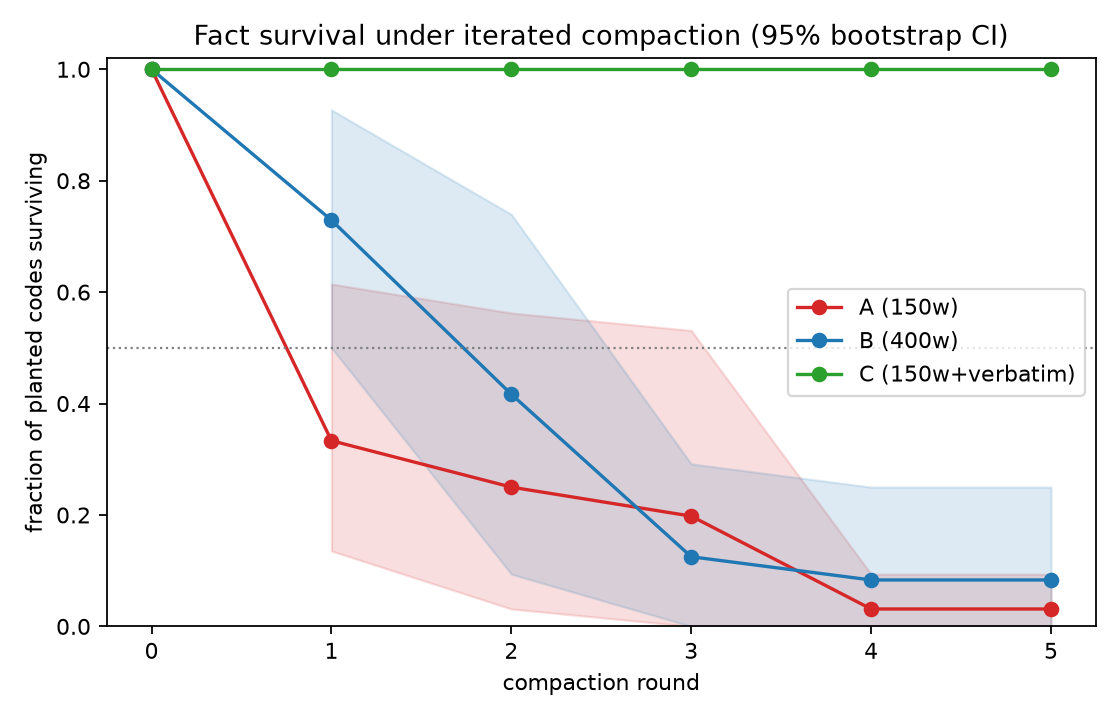
\includegraphics[width=0.85\linewidth]{retention_by_round.png}
\caption{Fact survival by compaction round, per arm, with 95\% bootstrap CIs
over chains.}
\label{fig:retention}
\end{figure}

\begin{figure}[t]
\centering
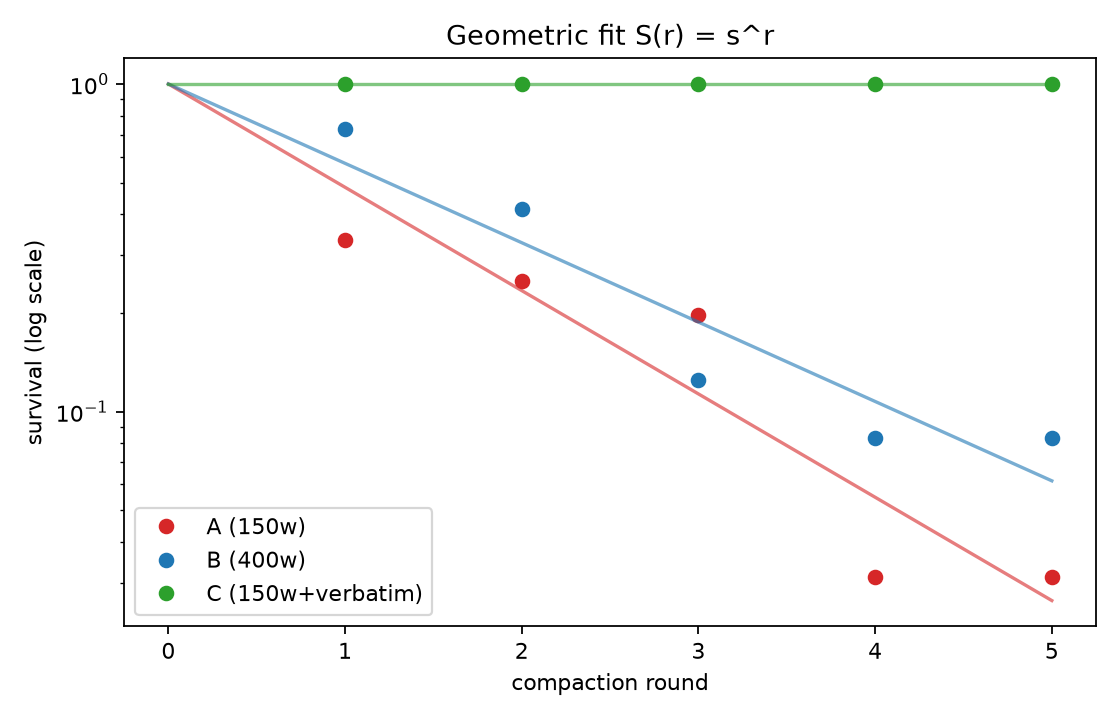
\includegraphics[width=0.85\linewidth]{survival_fit.png}
\caption{Geometric fit $S(r) = s^r$ on a log scale. Points are arm means;
lines are the pre-registered least-squares fits through the origin.}
\label{fig:fit}
\end{figure}

\subsection{H1: decay shape}

For no arm does the pre-registered $\delta$ rule call the decay front-loaded:
every 95\% bootstrap CI of $\delta$ includes 0. The data are therefore
consistent with geometric decay,
though the wide CIs mean this is a failure to reject rather than strong
evidence for constant per-round loss; Figure~\ref{fig:fit} shows visible
deviations from the fitted lines at this sample size.

\subsection{H2 and H3: budget vs.\ instruction}

Table~\ref{tab:contrasts} reports the pre-registered contrasts. H2 fails: the
400 vs.\ 150-word budget difference in round-5 survival is $\HTwoRfiveDiff$
(95\% CI $[\HTwoRfiveLo,\HTwoRfiveHi]$) and in fitted $s$ is $\HTwoSDiff$
$[\HTwoSLo,\HTwoSHi]$; neither CI excludes 0, so no budget effect is claimed at
round 5 despite Arm B's clear round-1 advantage. H3 succeeds decisively: the
verbatim instruction improves round-5 survival by $\HThreeRfiveDiff$
$[\HThreeRfiveLo,\HThreeRfiveHi]$ and fitted $s$ by $\HThreeSDiff$
$[\HThreeSLo,\HThreeSHi]$. Arm C also beats the 2.7$\times$ larger budget
directly ($\CBRfiveDiff$ round-5 survival, CI $[\CBRfiveLo,\CBRfiveHi]$), while
exceeding its own 150-word budget in only \ArmCOverBudget{} of 30 rounds (mean summary length
\ArmCMeanWords{} words vs.\ \ArmAMeanWords{} for Arm A and \ArmBMeanWords{} for
Arm B).

\subsection{Failure mode: clean loss, no corruption}

Across all \NCalls{} chain calls, \NMutated{} mutated codes were observed:
no summary ever contained a near-miss (edit distance 1--2) variant of a planted
code that was absent verbatim. Loss under compaction is availability loss
(facts silently omitted), not integrity loss (facts corrupted). The validation
probes reinforce this: asked questions answerable only from a round-5 summary,
the model answered the substring-retained code exactly
(\NProbeRetainedExact/\NProbeRetained) and, for substring-lost facts, answered
UNKNOWN in \NProbeAbstained{} of \NProbeLost{} cases with \NProbeConfab{}
code-like confabulations. The substring metric therefore tracks answerability
in both directions, and downstream consumers of a compacted context see missing
facts, not wrong facts.

\subsection{Position and content effects}

Survival is mildly position-dependent in the plain arms
(Figure~\ref{fig:position}: early-planted facts survive best), directionally consistent with
serial-position effects in long-context use \cite{liu2024lost}, though this
experiment is not powered to make positional claims. An exploratory,
non-pre-registered observation: during the pilot the model sometimes treated
credential-like values (passwords, tokens) as sensitive and redacted them
during recompaction; in the main data secret-like descriptors show no round-5
survival advantage in the plain arms. The verbatim instruction eliminated the
behavior in Arm C. This is flagged as exploratory only.

\begin{figure}[t]
\centering
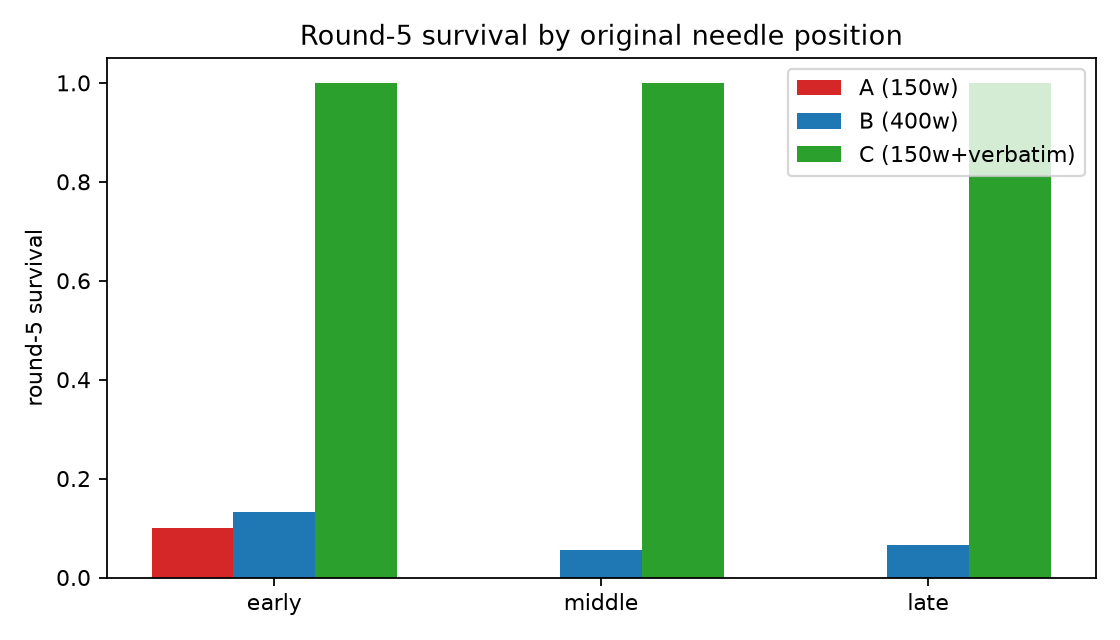
\includegraphics[width=0.85\linewidth]{position_survival.png}
\caption{Round-5 survival by the fact's original position tercile in the
round-0 source.}
\label{fig:position}
\end{figure}

\subsection{Variance and stability}

Chain-level variance is large. In Arms A and B, round-5 survivors concentrate
in single chains (one Arm B chain holds all \ArmBCntFive{} of that arm's
survivors). Table~\ref{tab:spotrepeat} shows the same chain spec run three
times: round-1 survival ranged from all 16 codes to none across runs. Point estimates for
individual chains are therefore highly unstable, echoing the unreliability
findings of \citet{laban2025lost}; only the arm-level contrasts with
chain-bootstrap CIs (Table~\ref{tab:contrasts}) should be trusted, and the
C-arm result is the only one large enough to clear that bar.

\section{Limitations}

Six chains per arm gives wide CIs; H2's null is a failure to detect, not
evidence of no effect. All results are from one small production model at one
date through one CLI harness; other models or scales may decay differently.
Facts are isolated random codes, which is the easy case for verbatim
preservation; entangled or paraphrasable knowledge may behave differently, and
a summary that keeps codes but drops their surrounding task state would still
score perfectly here. Arm C's perfect retention is a ceiling: with 16 facts and
5 rounds this design cannot distinguish truly lossless compaction from slow
decay, and sustaining verbatim retention at larger fact counts within a
150-word budget is impossible in principle. The run-to-run variance measurement
uses only 3 repeats of one spec. Finally, the geometric fit is a summary
statistic, not a mechanistic claim.

\section{Conclusion}

Under realistic iterated compaction, a small production model loses planted
facts with a half-life of roughly one to one-and-a-quarter compaction rounds,
and after five rounds retains almost nothing, regardless of whether the summary
budget is 150 or 400 words. A single added sentence demanding verbatim
preservation of identifiers moved retention from \ArmACntFive/96 to
\ArmCCntFive/96 at round 5 at essentially no cost in summary length. For
builders of long-running agents and memory systems
\cite{chhikara2025mem0,suzgun2025dynamic,zhang2025agentic}, the practical
takeaway is that what the compaction prompt asks for matters far more than how
much room the summary gets, and that losses are silent omissions, so anything
not explicitly protected should be assumed gone within a few compactions.

\paragraph{Reproducibility.} All chain specs, prompts, raw model responses,
scoring code, and the analysis pipeline that emits every number and table in
this paper are retained alongside the manuscript; the experiment cost
USD~\GrandCost{} in API calls.

\begin{table*}[t]\centering\footnotesize
\setlength{\tabcolsep}{2pt}
\caption{Fact survival $S(r)$ by arm (mean over 6 chains, 95\% bootstrap CI over chains, 10{,}000 reps), fitted per-round survival constant $s$, and compaction half-life in rounds.}
\label{tab:survival}
\begin{tabular}{lccccccc}
\toprule
Arm & $S(1)$ & $S(2)$ & $S(3)$ & $S(4)$ & $S(5)$ & $s$ & half-life \\
\midrule
A: 150w & 0.33 [0.14,0.62] & 0.25 [0.03,0.56] & 0.20 [0.00,0.53] & 0.03 [0.00,0.09] & 0.03 [0.00,0.09] & 0.484 & 0.95 \\
B: 400w & 0.73 [0.50,0.93] & 0.42 [0.09,0.75] & 0.12 [0.00,0.29] & 0.08 [0.00,0.25] & 0.08 [0.00,0.25] & 0.573 & 1.24 \\
C: 150w+verbatim & 1.00 [1.00,1.00] & 1.00 [1.00,1.00] & 1.00 [1.00,1.00] & 1.00 [1.00,1.00] & 1.00 [1.00,1.00] & 1.000 & $>$100 \\
\bottomrule
\end{tabular}
\end{table*}

\begin{table}[t]\centering\small
\caption{Pre-registered arm contrasts. Difference and 95\% bootstrap CI (chains resampled independently per arm, 10{,}000 reps); a difference is claimed only if the CI excludes 0.}
\label{tab:contrasts}
\begin{tabular}{llccc}
\toprule
Contrast & Metric & Diff & 95\% CI & Claimed \\
\midrule
H2: B $-$ A & round-5 survival & $+0.052$ & $[-0.062,+0.250]$ & no \\
H2: B $-$ A & fitted $s$ & $+0.089$ & $[-0.320,+0.460]$ & no \\
H3: C $-$ A & round-5 survival & $+0.969$ & $[+0.906,+1.000]$ & yes \\
H3: C $-$ A & fitted $s$ & $+0.516$ & $[+0.411,+0.807]$ & yes \\
C $-$ B & round-5 survival & $+0.917$ & $[+0.750,+1.000]$ & yes \\
\bottomrule
\end{tabular}
\end{table}

\begin{table}[t]\centering\small
\caption{Run-to-run stability: the identical chain spec (A-0) run three times with fresh model calls. Surviving codes out of 16 by round.}
\label{tab:spotrepeat}
\begin{tabular}{lccccc}
\toprule
Run & $r{=}1$ & $r{=}2$ & $r{=}3$ & $r{=}4$ & $r{=}5$ \\
\midrule
A-0 & 16 & 16 & 16 & 0 & 0 \\
repA0-rep1 & 0 & 0 & 0 & 0 & 0 \\
repA0-rep2 & 4 & 2 & 2 & 2 & 2 \\
\bottomrule
\end{tabular}
\end{table}


\bibliographystyle{plainnat}
\bibliography{references}

\end{document}
